%% LyX 2.2.2 created this file.  For more info, see http://www.lyx.org/.
%% Do not edit unless you really know what you are doing.
\documentclass[english]{article}
\usepackage[T1]{fontenc}
\usepackage[latin9]{inputenc}
\usepackage{array}
\usepackage{float}
\usepackage{rotfloat}
\usepackage{graphicx}

\makeatletter

%%%%%%%%%%%%%%%%%%%%%%%%%%%%%% LyX specific LaTeX commands.
%% Because html converters don't know tabularnewline
\providecommand{\tabularnewline}{\\}

\makeatother

\usepackage{babel}
\begin{document}

\title{Online Appendix: Measuring the Landscape of Civil War (v1.0)}

\date{December 2017}

\author{Dr. Rex W. Douglass\\
 University of California, San Diego\\
 \\
 Dr. Kristen A. Harkness\\
 University of St. Andrews\\
 kh81@st-andrews.ac.uk }

\maketitle
This online appendix accompanies the paper ``Measuring the Landscape
of Civil War: Evaluating Geographic Coding Decisions with Historic
Data from the Mau Mau Rebellion.'' It is intended to provide greater
technical detail than was within the scope of the original article.
Please visit the online repository (available here{[}\footnote{https://github.com/rexdouglass/MeasuringLandscape}{]})
for the most up to date version of this document as well as full technical
replication material for the paper.

\tableofcontents{}

\section{Introduction}

\section{``Best Practices and New Tools for Building Geographic Conflict
Data''}

\subsection{``Which Coordinate Sources?''}

\subsubsection{Gazetteers}

We employ a number of different gazeteer sources for this analysis
including:
\begin{enumerate}
\item The 1964 Official Kenya Gazetteer (United States Board of Geographic
Names, 1964);
\item The U.S. Board of Geographic Names\textquoteright{} database of foreign
geographic feature names or NGA (http://geonames.nga.mil/gns/html/namefiles.html);
\item The National GeospatialIntelligence Agency\textquoteright s GeoNet
Names Server or GeoNames (http://download.geonames.org/export/dump;
\item Google Maps\textquoteright{} search API;
\item Bing Maps\textquoteright{} search API;
\item OpenStreetMap (Kenya extract retrieved from http://download.geofabrik.de/africa.html);
\item Global Administrative Areas database or GADM (http://www.gadm.org); 
\item Getty Thesaurus of Geographic Names (http://www.getty.edu/research/tools/vocabularies/tgn/index.html);
\item International Livestock Research Institute (http://192.156.137.110/gis/search.asp?id=386); 
\item Wikidata (https://www.wikidata.org).
\end{enumerate}

\subsubsection{Gazetteer Coverage}

We subset each gazeteer to just the region of interest covering the
conflict. As you can see, the spatial coverage varied wildly from
source to source, with some like Geonames having very densive coverage
of this area to others like Openstreetmap having relatively sparse
coverage. Coverage for both Google and Bing map APIs is based on just
the set of entities returned when searching for the toponyms in our
events data, not their full coverage of this area. 

\begin{figure}
\hfill{}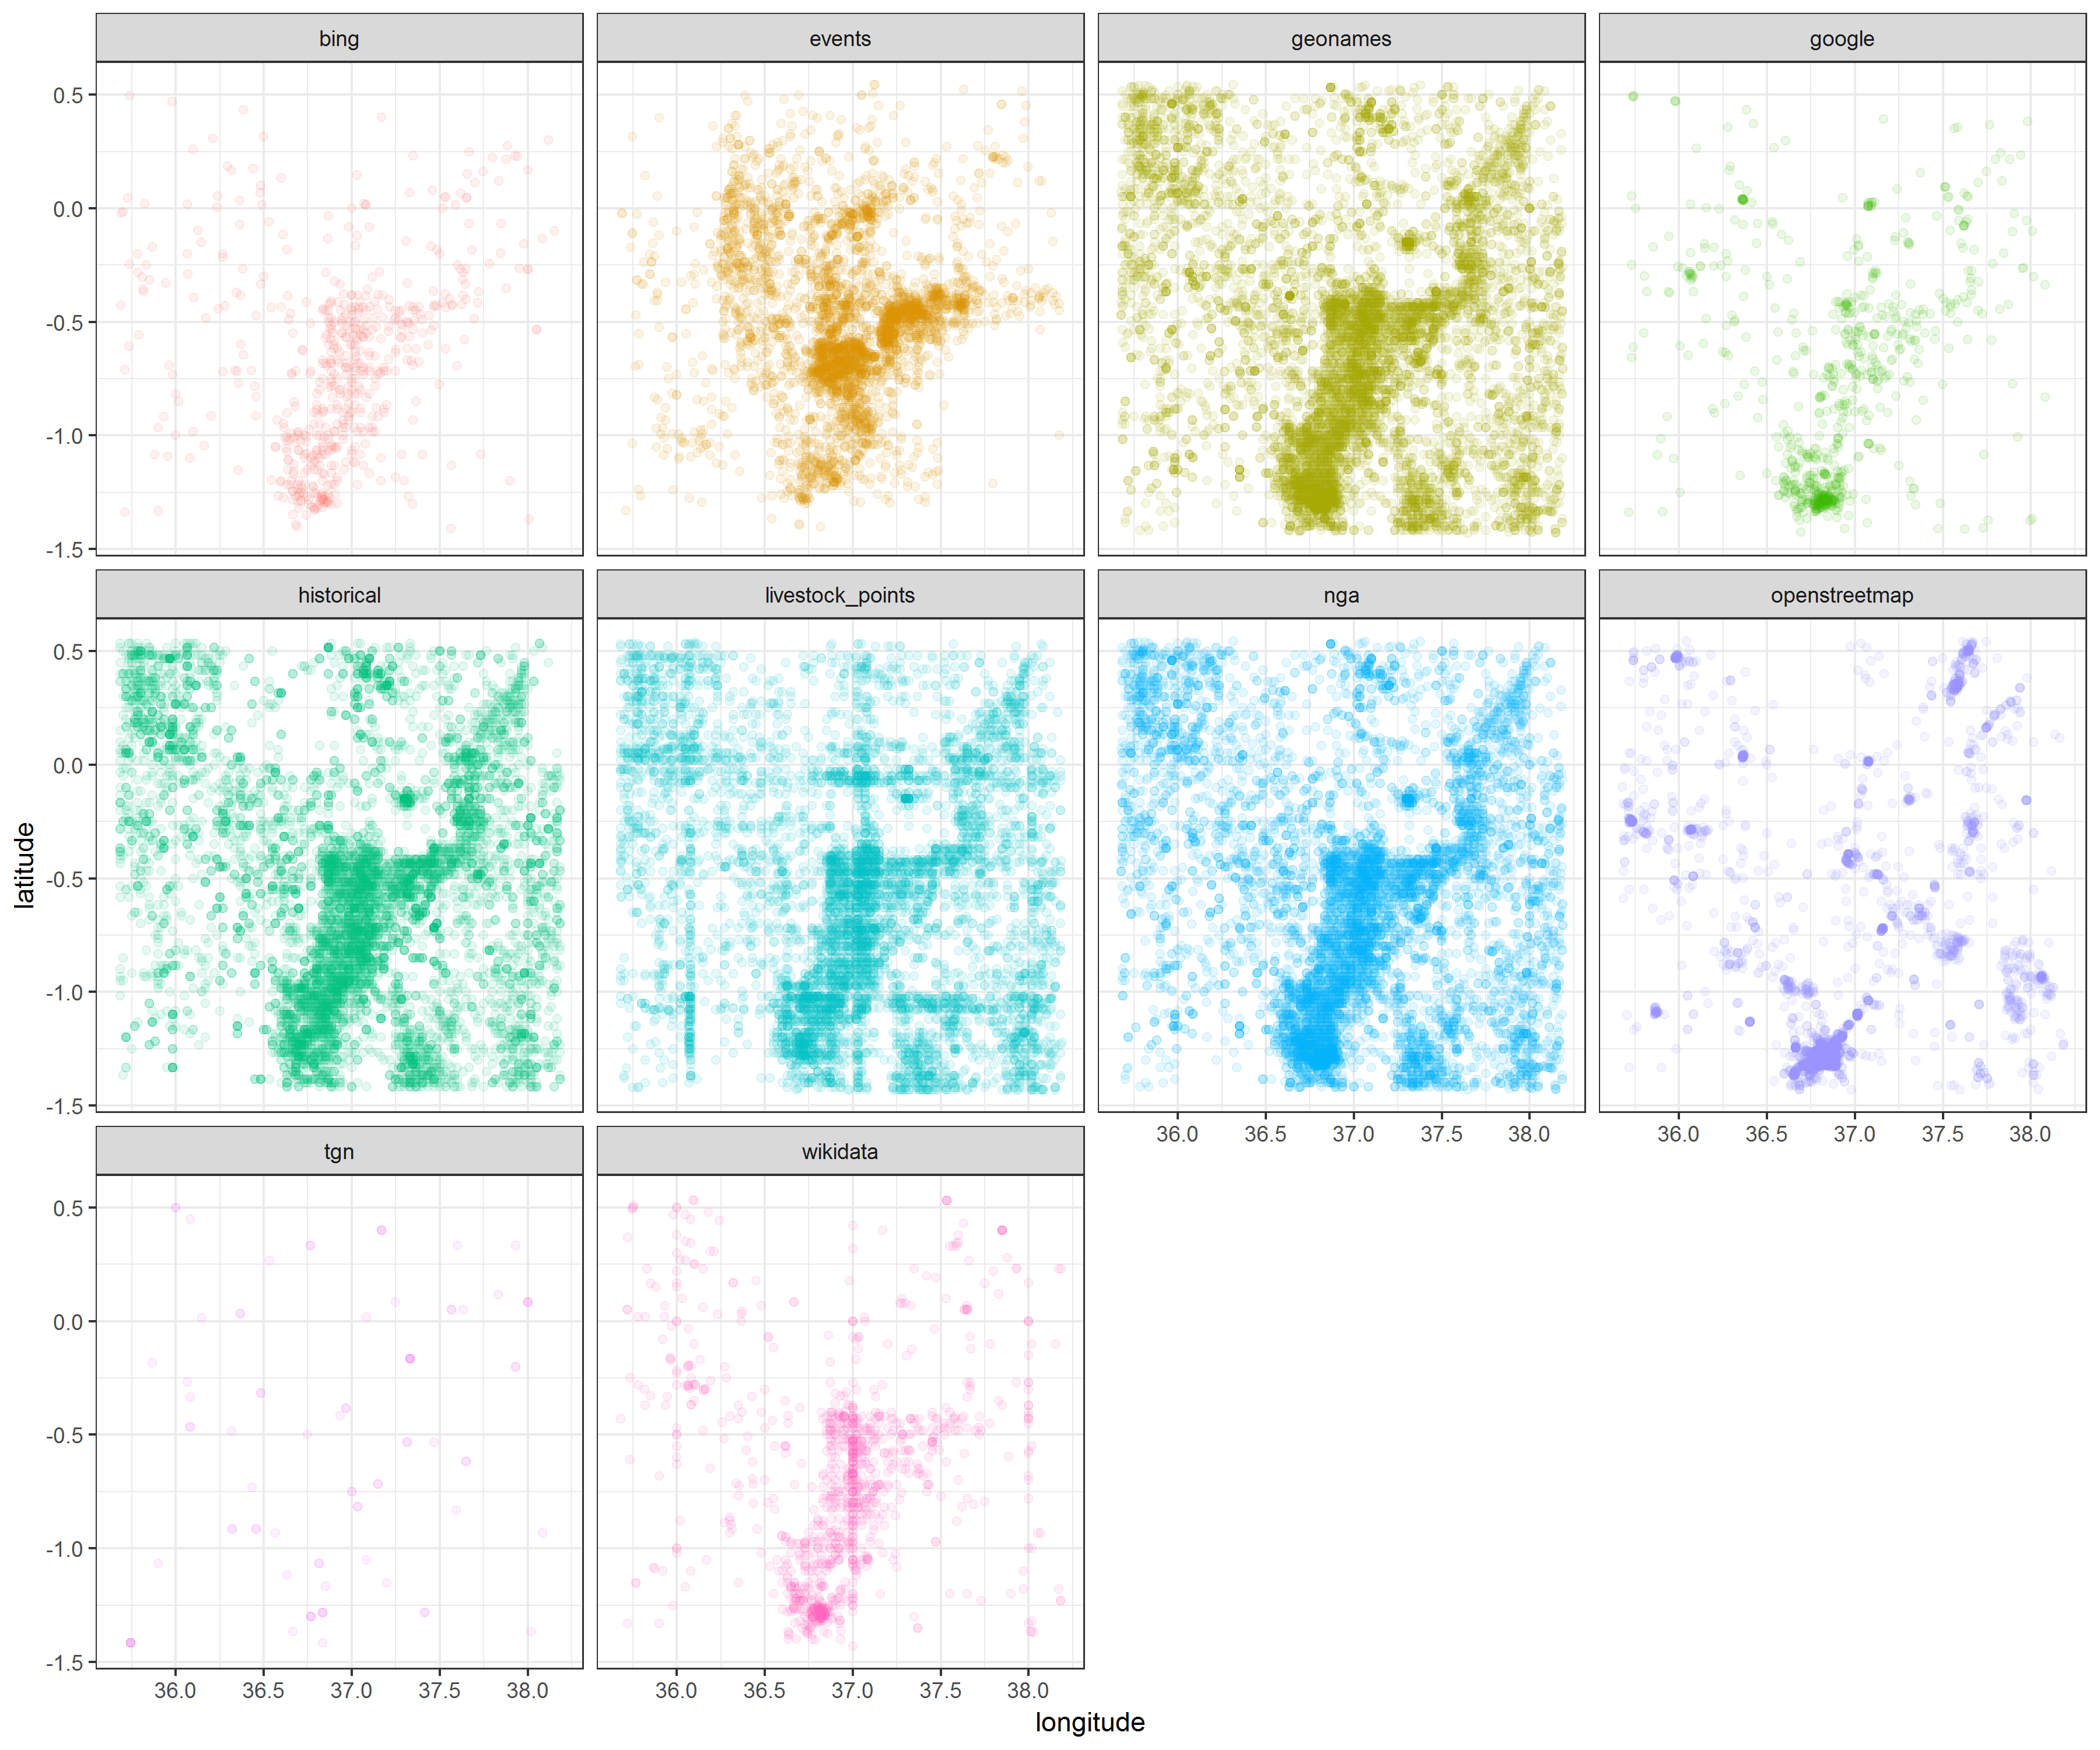
\includegraphics[width=5.5in]{figures/flatfiles_sf_roi_facet_source_dataset_points}\hfill{}

\caption{Spatial coverage within the region of interest of nine gazeteer sources
that have point features.}
\end{figure}


\subsubsection{Gazetteer Resolution}

Each source has an implicit spatial resolution based on how it was
created and whether and how those coordinates were translated (e.g.
from degrees to decimal). By far the worst source was the digitization
effort of the livestock, with both coarse precision and noticeable
artifacts of points lying directly on latitude and longitude map lines
which were omitted or pushed to the side. The historical gazetteer
was presented in minutes and seconds, limiting its maximum precision
to about 2km on the ground. NGA and geonames are a combination of
the historical gazetteer as well as new points drawn from other sources
with a plausibly higher resolution. Openstreetmap is drawn directly
on satellite imagery by humans, but also imports some off the shelf
data. Wikidata has a noticeable truncation to the whole degree. Our
events locations have a known spatial resolution at the grid square,
which our conversion to latitude/longitude gives a smooth but false
sense of accuracy. In sum, we recommend a bounding box of 2km around
any point.

\begin{figure}
\hfill{}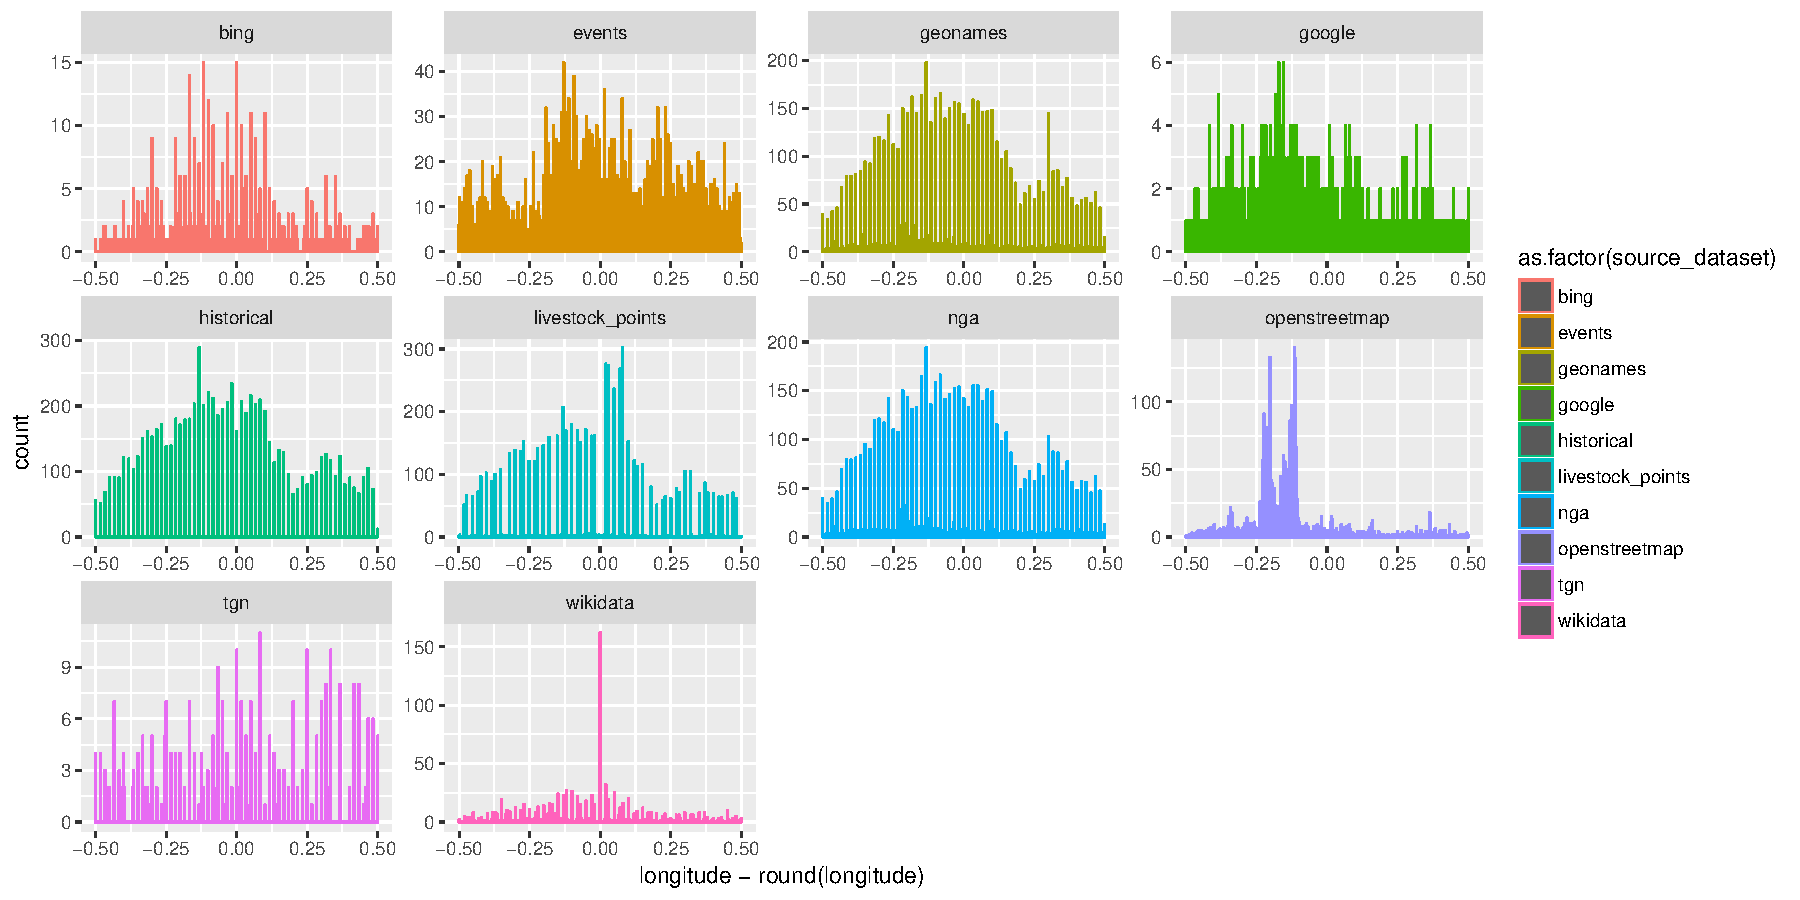
\includegraphics[width=5.5in]{figures/p_combs_long}\hfill{}

\caption{Histogram of longitude coordinates.}
\end{figure}


\subsection{``Allow Self-Referential Matching?''}

\subsection{``Which Geometry Type''}

\begin{figure}
\hfill{}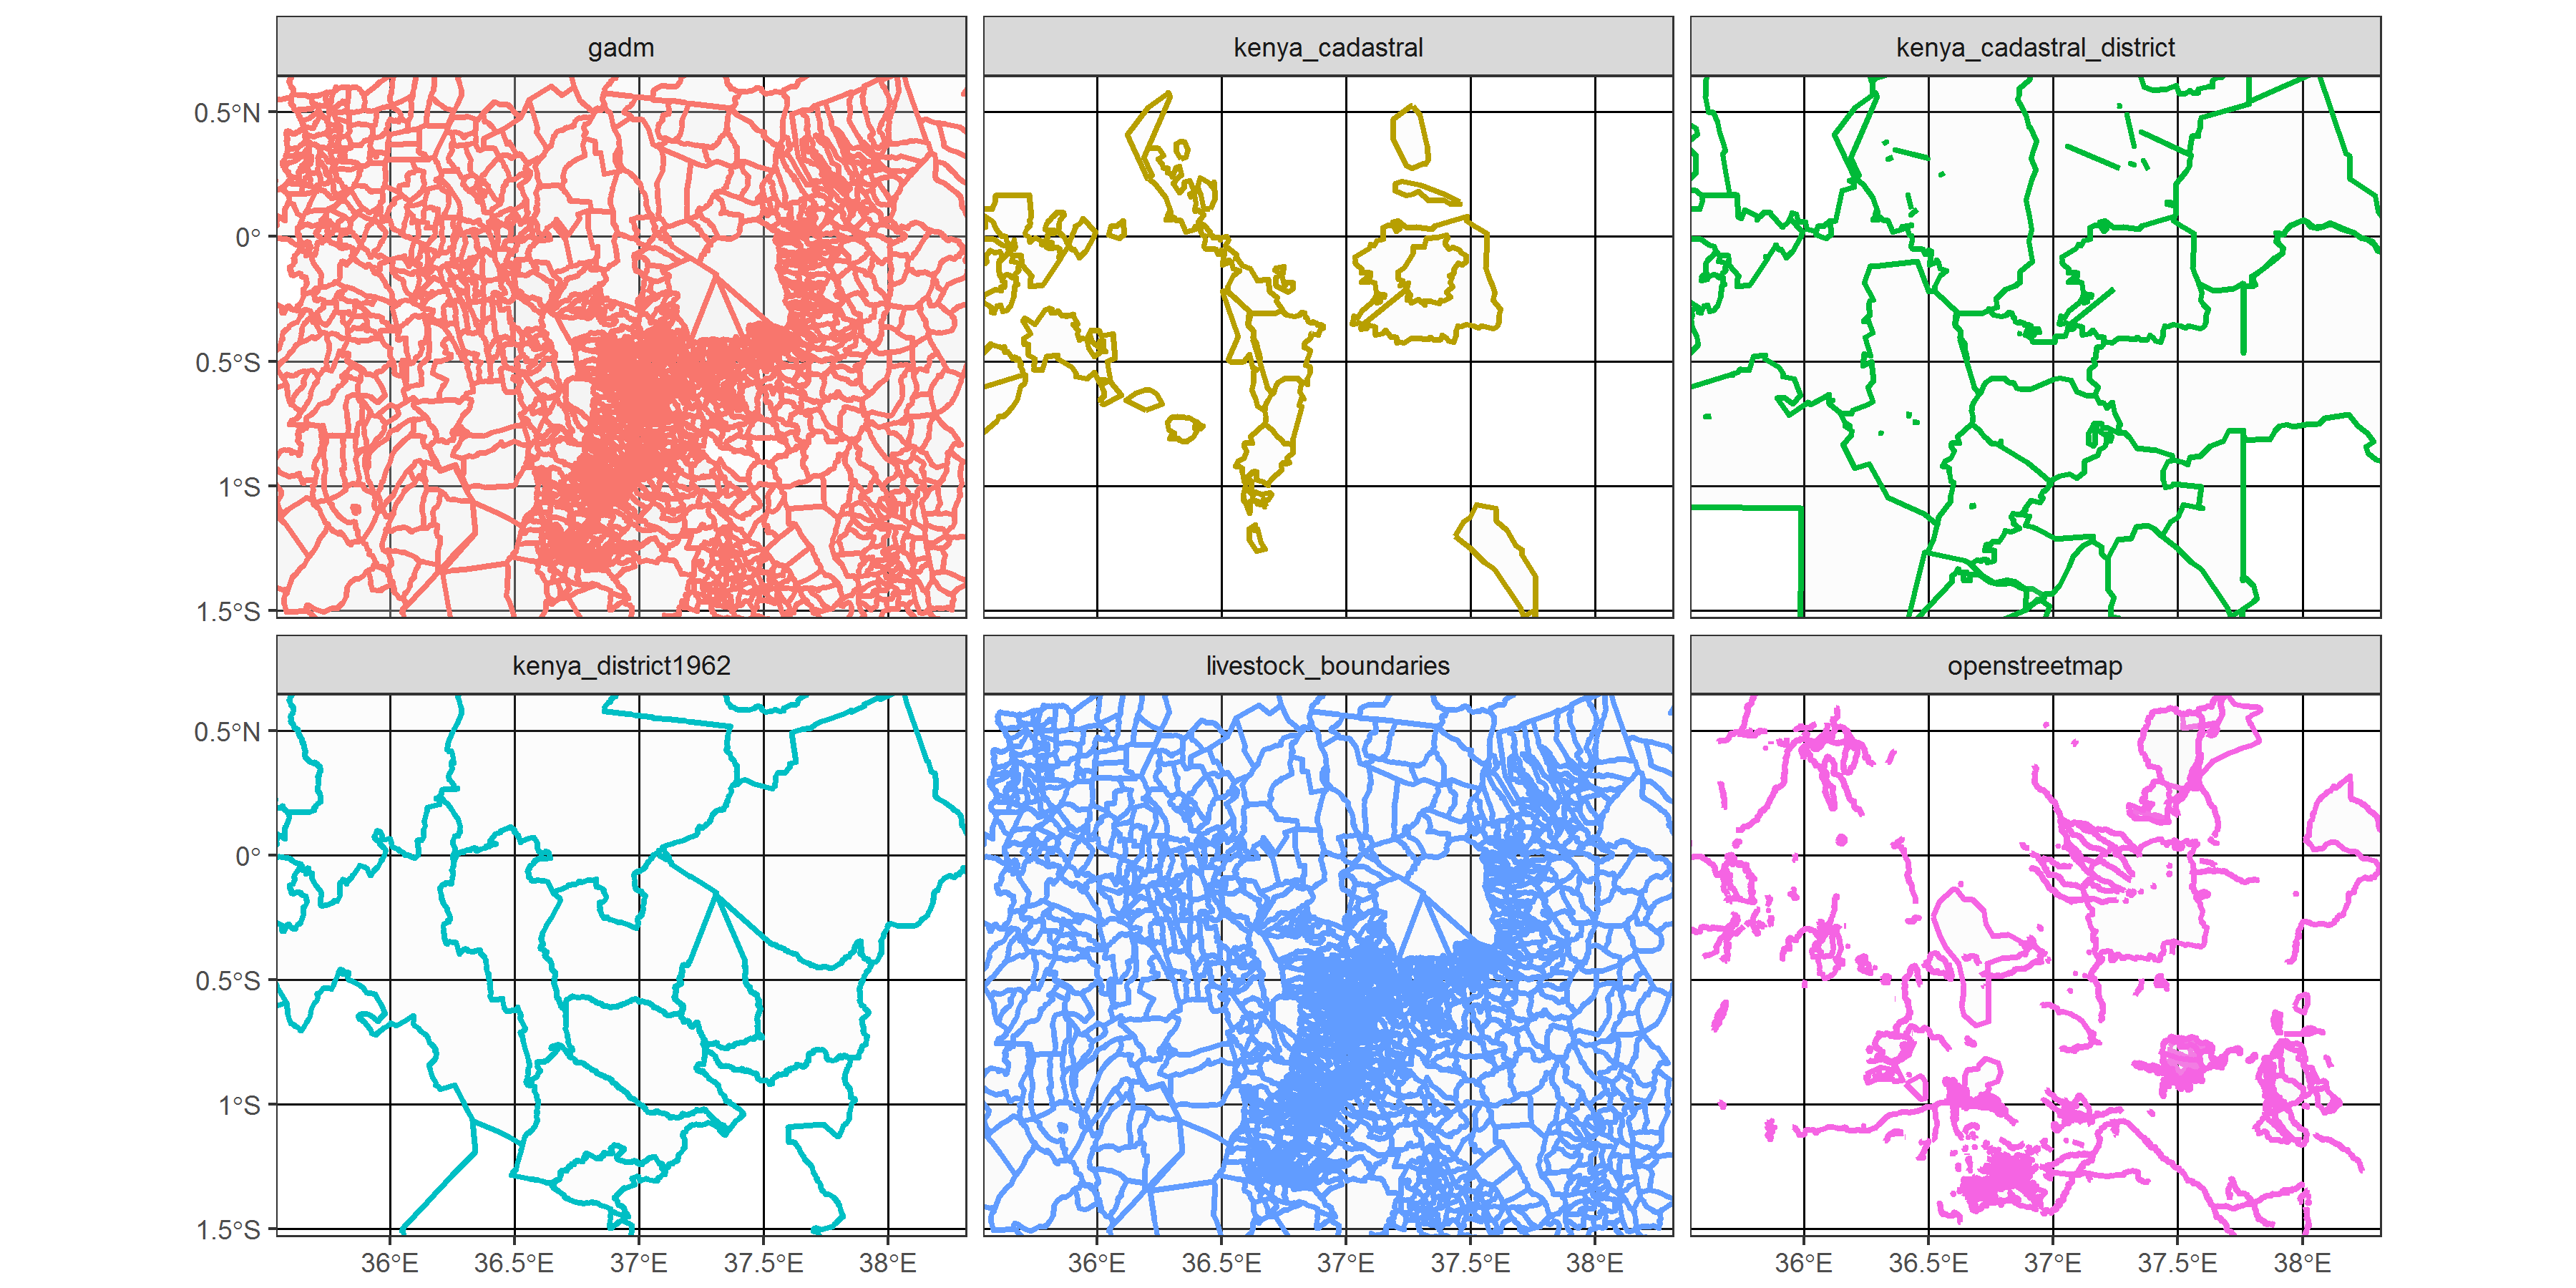
\includegraphics[width=5.5in]{figures/flatfiles_sf_roi_facet_source_dataset_notpoints}\hfill{}

\caption{Histogram of longitude coordinates.}
\end{figure}


\subsection{``Type of String Matching''}

We introduce the concept of fuzzy matching but do describe the approach
in great detail. Our fuzzy matching pipeline has three major steps,
stemming, locally sensitive hashing, and a supervised classifier.

\subsubsection{The Problem}

When comparing two toponyms, how should we decide when they are referring
to the same real world location and when they are actually referring
two different real world locations? This is a difficult task for several
reasons. The first is that relatively little information is conveyed
by a string alone outside of the context in which it was used, e.g.
the word ``Paris'' is not enough to uniquely distinguish between
a vacation to Paris, France or a one to Paris, Texas. Second, the
way topynms are used (and abused) in natural language text leads to
many different unique strings referring to the same underlying toponym.
We have enumerated just some of the ways toponyms are misrepresented
in natural language text in our event data, shown in columns one and
two of the table below.

\begin{table}
\hfill{}%
\begin{tabular}{|>{\centering}p{1in}|>{\centering}p{2.5in}|}
\hline 
{\small{}Variant} & {\small{}Examples}\tabularnewline
\hline 
\hline 
\textbf{\small{}Nonnames} & \tabularnewline
\hline 
\textbf{\small{}Personal Names} & {\small{}a.e.aggatt's farm; buckley's road; count van der stegen;
lady eleanor cole's farm at elmentetia}\tabularnewline
\hline 
\textbf{\small{}Near Spellings Same} & {\small{}Burguret Estate;Burgaret Estate;Burgaret Entate }\tabularnewline
\hline 
\textbf{\small{}Near Spellings Different} & {\small{}s.e.bastard; S.S. Bastard's Farm}\tabularnewline
\hline 
\textbf{\small{}Directional} & {\small{}1 mile w.of bariaho; between eburru and kipipiri; between
slaters and salisbury road; border of the iriaini \& magutu, iriaini;
embu/ south nyeri border; footpath leading to muthara; marula estate
near longonot}\tabularnewline
\hline 
\textbf{\small{}Synonyms} & {\small{}aberdare forest; aberdare forest reserve}\tabularnewline
\hline 
\textbf{\small{}Supranational Information} & {\small{}aberdares f.hall; bentall's farm, nakuru; col.culton house
kon-gaita}\tabularnewline
\hline 
\textbf{\small{}Abbreviations} & {\small{}aguthi loc s.n.r; clarke's fm.; gura rv.; malik s/mills;
nr githumu}\tabularnewline
\hline 
\textbf{\small{}Corporate Names} & {\small{}blue post hotel}\tabularnewline
\hline 
\textbf{\small{}Ambiguous} & \tabularnewline
\hline 
\textbf{\small{}Spelling Errors} & {\small{}chehe sow mills; nairobi south esp llabour line}\tabularnewline
\hline 
\textbf{\small{}Contemporary Context} & {\small{}chief hinga's location; chief makimeis and waruiru's location;
forest loc 14}\tabularnewline
\hline 
\textbf{\small{}Compound Locations} & {\small{}cole estates, gamble's farm}\tabularnewline
\hline 
\textbf{\small{}Grid Locations} & {\small{}eastings 43-47, northings 34-35}\tabularnewline
\hline 
\textbf{\small{}Sub-Information} & {\small{}eastleigh section 7}\tabularnewline
\hline 
\textbf{\small{}Compound Names} & {\small{}fort hall / thika road; gakurwa loc 14/15}\tabularnewline
\hline 
\textbf{\small{}Punctuation} & {\small{}luis farm; luis' farm}\tabularnewline
\hline 
\textbf{\small{}Numeric Postfix Irrelevant} & {\small{}marmanet mill no1}\tabularnewline
\hline 
\textbf{\small{}Numeric Postfix Relevant} & {\small{}Location 1; Location 11}\tabularnewline
\hline 
\textbf{\small{}Additional information} & {\small{}loc 8 fort hall}\tabularnewline
\hline 
\textbf{\small{}Directional Potfixes} & {\small{}mathira north; mathira south}\tabularnewline
\hline 
\textbf{\small{}Missing spaces} & {\small{}murandialocation 8}\tabularnewline
\hline 
\end{tabular}\hfill{}

\caption{Example natural language descriptions of toponyms.}
\end{table}

\begin{sidewaystable}
\hfill{}%
\begin{tabular}{|c|>{\centering}p{1.5in}|>{\centering}p{2in}|>{\centering}p{2in}|>{\centering}p{2in}|}
\hline 
 & Events & gazeteers & News Corpus & Issues\tabularnewline
\hline 
\hline 
``Ol Kalou''  & ``OLKALOU'', ``OL KALOU'',''Mark's farm OLKALOU'',''KALOU TOWNSHIP'',''KALOU'',''01
KALOU TOWNSHIP'',''01 KALOU FLATS'', and ``01 KALOU'' & ``Ol Kalou'' (PPLA, PPL, locality;political, PopulatedPlace, town,
railway\_station, Trading Centre)

``Olkalou Country Club'' (SOCF), 

``olkalou'' (locality;political),

''ol kalou flat'' (locality;politica),''

''kalou'' (locality;political)

``Ol Kalou Road'' (unclassified) & kalou, o1 kalou, o kalou, o'kalou, ol kalou, oikalou, oi kalou, olkalou,
okalou, kalou salient, kalou route, kalou hospital, kalou township,
o'kalou plot, township of olkalou, kalou district, olkalou township,
okalou plot, o1 kalou route, kalou west, kalou central, kalou nyandarua
district, kalou road, oil kalou, oikalou hospital, kalou hospital
nyandarua, kalou south, alou town, oj kalou, ol kalou township, township
of olkalou township, kalou location, township of ol kalou, kalou naivasha
district, o kalou salient, oi'kalou, ol kalou location  & Consolidating different spellings and errors. Misspellings occur frequently
in news corpus also.

Levels of aggregation that appear in news corpus but not gazeteers
(e.g. location, distric). \tabularnewline
\hline 
``BASTARD'' & W.K. BASTARD'S PUMP HOUSE, W.K. BASTARD'S FARM, S.S.Bastard's Farm
Nanyuki, S.S.Bastard's Farm,S.K.Bastard, Kongai R.W.K.Bastard, HUTCHINSON'S
FARM, S.S BASTARDS FARM, BASTARD'S FARM & NONE! & bastard, s bastard, bastard esq, k bastard, w k bastard, k bastard
esq, w k bastard esq, s s bastard, nanyuki bastard, bastard william,
w s bastard, bastard esq po, h s bastard, s bastard esq, hs bastard,
kenneth bastard, bastard s, william kenneth bastard, bastard esq farm,
bastard esq nanyuki, bastard esq sw estate,  & Zero gazeteer matches. Relying on coordinates from other events. Common
surname Bastard applies to multiple households. Surname alone isn't
sufficient to disambiguate which.\tabularnewline
\hline 
Nairobi & THIKA/NAIROBI ROAD,R NAIROBI GOLF CLUB , NAIROBI/NAKURU, NAIROBI WEST,
Nairobi South E.A.P \& L.Labour Line , NAIROBI SOUTH, NAIROBI RIVER,
NAIROBI DAM, NAIROBI DAM, NAIROBI CITY, NAIROBI, KIAMBU, NAIROBI & 464 matches... Nairobi, Nairobi City, Nairobi City County, Nairobi
National Park, 2011 Nairobi pipeline fire, Bahati, Nairobi, Nairobi
- Mombasa Railway, Nairobi - Nakuru Road, Nairobi / Dagoretti, NAIROBI
AIRPORT &  & No events with Nairobi provide coordinates to verify strategy. Extreme
number of gazetteer matches all over the country. Extreme number of
text matches.\tabularnewline
\hline 
\end{tabular}\hfill{}

\caption{Example toponym variations across sources.}
\end{sidewaystable}


\subsubsection{Training Data}

We treat this a supervised learning problem and develop a hand labeled
dataset of toponym matches (3,192) and mismatches (17,051). We construct
a training dataset by taking the 5,128 events with both text and coordinates
and pairing them with the ten gazetteer entries closest in geographic
proximity, for 51,280 event-gazetteer diads. To avoid weighting locations
with more events, we only keep one unique example of each location
description-gazetteer toponym diad. We further exclude exact matches
with identical text on both sides, leaving 20,242 diads to consider.
We create a training split (80\%) and testing split (20\%) witheld
only for evaluating model performance by selecting 500 random toponym
stems and excluding any diad with the stem on either pole. 

\subsubsection{Stemming}

Toponyms often include a mix of uniquely identifying tokens (stems)
and generic place type descriptions (postfixes) like ``farm'', ``estate'',
``hospital'', etc. This creates a problem for string matching for
two reasons. First, postfixes are not used consistently, appearing
in some entries for the same place but not others. Second, postifixes
make toponyms look similar because of their type but not necessarily
their geography. We therefore develop a rule based toponym stemmer.
We took the 14,885,300 unique names and alternate names, stripped
off the first word of each, leaving 8,740,662 unique suffixes. To
account for multiword stems and to ensure we capture broadly applicable
postfixes we further require them to appear at least 5 times, resulting
in 161,034 unique postfixes. For example, the five most common postfixes
globally are ``creek'' (63,214), ``lake'' (40,595), ``river''
(36,379), ``island'' (31,347), ``well'' (30,091), ``point''
(28,225), and ``cemetery'' (27,345). Across the 57,903 unique toponyms/descriptions
across both the events and combined gazeteers, we find 45,131 unique
stems, and 2,546 unique postfixes.

\subsubsection{Locally Sensitive Hashing}

Unfortunately, the number of pairwise comparisons that must be made
scales quadradically in the number of items, over a billion comparisons
for our moderately sized dataset (k\textasciicircum{}2 / 2 = 45,131
stems\textasciicircum{}2 / 2= 1,018,403,580), and so using only exact
comparisons is impractical. We therefore introduce an intermediate
culling stage based on approximate matching. The suggester's goal
is to strike a balance that minimizes the number of false negatives
at the cost of a reasonable number of false positives. The approach
we employ is called Locality Sensitive Hashing (LSH), and it proceeds
in two steps (Leskovec et al. 2010, chapter 3). First, we convert
each toponym into a standardized sparse vector of binary features.
Q-gram distance performed well for both the matcher and so we choose
q-gram profiles as our sparse feature set.\footnote{Grams are simply counts of characters \{'a','b','1'\}, pairs of characters
\{'ed','ac'\} , sets of three characters in a row \{'abc','ing'\},
etc. Skip grams extend this idea to allower for gaps between pairs
or tripplets, e.g. \{'a\_c','c\_e'\}, etc.} The similarity between any two profiles is measured as the Jaccard
distance which is the just the count of shared items in both sets
divided by the total number of items in both. To avoid having to calculate
that distance for every single pair of items, we apply a hash function
that assigns two items to the same id with some probability as a function
of their jaccard distance. By using multiple hashes, one can choose
an arbitrary threshold for which items below a certain distance will
be matched with very high likelihood. The advantage is this procedure
only requires a single pass through the entire set of items. The downside
is it provides only a hard yes or no match, and there is a trade off
between retrieving too many suggestions and losing too many real matches
which must be hand tuned. Using the hand labeled training data, we
experimentally determined the optimal combination of gram features,
and hash hyperparameters. We settled on 1-grams, 2-grams, and 2-grams
with a single skip, and LHS parameters of 400 bands with 5 rows. This
produced a recall rate of 0.95 at the cost of an average of 72 suggestions
per item. That reduces the number of comparisons we need to evaluate
for the full dataset from over a billion to just over three million,
a 99.7\% reduction. Those pairs that pass the suggester's bar then
go on to the matcher for further refinement and a direct estimate
of the likelihood of a match.

\begin{figure}
\hfill{}\hfill{}

\caption{}
\end{figure}


\subsubsection{Fuzzy Matcher}

We train a classifier to predict the likelihood of match between two
toponyms as a function of properties of each. We consider both the
full strings and also their stems. For each, we employ nine types
of string distance (Jaro, Optimal String Alignment, Levenstein, Damerau
Levenshtein, Longest Common Substring, q-grams 1-5, cosine, Jaccard,
and a count of the number of matching letters before the first mismatch).
We include a count of the number of characters of A and B and the
difference between the lengths. We also consider the context of each
string as represented in Kenya Gazetter including the number of times
mentioned total, the minimum, mean, median, and max years in which
it was mentioned.

The classifier we employ is tree based gradient boosting algorithm
called Extreme Gradient Boosting (XGBoost) (Chen et al. 2016). The
method, in brief, is a greedy function aproximator, additively combining
multiple functions, that are estimated one at a time, each seeking
to account for the residuals of the prior functions (Friedman 2001).
 In our case, each function is approximated by a nonparemtric decision
tree which starts at a root node containing every observation, and
progressively splits observations into purer and purer subsets using
cut points along their covariates. We employ a custom loss function,
seeking to minimize the log likelihood. We account for the class imbalance
by proportionally weighting positive and negative cases. To avoid
over-fitting, we use early stopping, based on area under the receiver
operating characteristic curve (AUC) on the test set. We observe convergence
at about 318 iterations.

The model performs well, with a classification error rate of 0.016.
The errors are balanced across classes, with an F-score of 0.99, and
AUC of 0.997, and an area under the Precision Recall Curve of 0.95.
Five features contribute disproportionately, all string distance measures,
Jaro Distance, q-gram 2, First Mismatch, Optimal String Alignment
(Unormalized), and q-gram 3. Through combining different string distance
measures, the model is deriving ways in which two strings might match,
by both starting with the same word, sharing long substring toward
the end, requiring small spelling changes to match, etc.

\paragraph{String Distance Measures}

We employ a number of string distance measures as features (Santos
et al. 2017), described in the table below.

\begin{table}
\hfill{}%
\begin{tabular}{|c|>{\centering}p{3in}|}
\hline 
Feature & \tabularnewline
\hline 
\hline 
First Mismatch & Counts the number of exact matching characters from the beginning
of each string\tabularnewline
\hline 
Cosine Distance & The cosine distance (method='cosine') is computed as 1-x\textbackslash{}cdot
y/(\textbackslash{}|x\textbackslash{}|\textbackslash{}|y\textbackslash{}|),
where x and y were defined above.\tabularnewline
\hline 
Levenshtein distance & The Levenshtein distance (method='lv') counts the number of deletions,
insertions and substitutions necessary to turn b into a. \tabularnewline
\hline 
Optimal String Alignment distance & Like the Levenshtein distance but also allows transposition of adjacent
characters. Here, each substring may be edited only once.\tabularnewline
\hline 
Full Damerau-Levensthein distance & Is like the optimal string alignment distance except that it allows
for multiple edits on substrings.\tabularnewline
\hline 
longest common substring & The lcs-distance is defined as the number of unpaired characters.
The distance is equivalent to the edit distance allowing only deletions
and insertions, each with weight one.\tabularnewline
\hline 
Jaro distance & The Jaro distance is defined as 1-(1/3)(w\_1m/|a| + w\_2m/|b| + w\_3(m-t)/m).
Here,|a| indicates the number of characters in a, m is the number
of character matches and t the number of transpositions of matching
characters. \tabularnewline
\hline 
\end{tabular}\hfill{}

\caption{Linker Features. Descriptions taken from the stringdist R package.}
\end{table}


\section*{``Ensembles''}

\subsection*{``Hand Rule Ensemble''}

\subsection*{``Supervised Ensemble''}

We introduce a supervised learning approach to choosing the optimal
gazeteer match. 

Model: XGBoost implemented in the R package xgboost (Chen et al. 2016).

Unit of Observation: Event place description - Potential Gazeteer
Match

N:= 468,046

Features: Gazeteer source, geometry type, fuzzy or exact string match,
and self reference; reporting district, the year of the event, and
what level geographic aggregation the event was reported at, e.g.
city, district, or province level.

Loss: Mean square error

Early stopping after 10 rounds, convering in 13 iterations.

Five fold cross validation with approximately equal hold out sets
divided by event location description to prevent the same name from
appearing in both training and test splits.

Out of sample error: root mean squared error of 1.088 log km.

\begin{figure}
\hfill{}\hfill{}

\caption{Variable Importance Plot for XGBoost model predicting distance between
observed location and each gazetteer match.}
\end{figure}


\section{Evaluating the Consequences of Georeferencing Decisions}

\subsection{\textit{Recall and Accuracy}}

In the main paper we present the average accuracy of each gazeteer
source in terms of mean squared distance. Here we present the cumulative
distributions of each sources shortest possible match, regardless
of name, to the observed military coordinate. This represent a hard
bound for a source's coverage, there are not any points of any kind
from the source closer than the stated distance that could even possibly
be a match given a name.

\begin{figure}[H]
\hfill{}\hfill{}

\caption{The CDF line for polygon matches from any gazeteer is lower in places,
because it matches more with lower average accuracy.}
\end{figure}


\section{Bias Estimates}

Each bias estimate is the result of an individual model fit to the
subset of points meeting the criteria described in the text. Not described
in the text are the hyper-parameters of the XGBoost model employed,
which are as follows.

Model: XGBoost implemented in the R package xgboost (Chen et al. 2016).

Unit of Observation: Event place description - Potential Gazeteer
Match

N:= 468,046

Features: Gazeteer source, geometry type, fuzzy or exact string match,
and self reference; reporting district, the year of the event, and
what level geographic aggregation the event was reported at, e.g.
city, district, or province level.

Loss: Log Loss with proportionally weighted cases to account for class
imbalance.

Five fold cross validation with random hold out sets.
\begin{thebibliography}{1}
\bibitem{key-1}Chen, Tianqi, and Carlos Guestrin. \textquotedbl{}Xgboost:
A scalable tree boosting system.\textquotedbl{} In Proceedings of
the 22nd acm sigkdd international conference on knowledge discovery
and data mining, pp. 785-794. ACM, 2016.

\bibitem{key-2}Leskovec, Jure, Anand Rajaraman, and Jeffrey David
Ullman. Mining of massive datasets. Cambridge university press, 2014.

\bibitem{key-3}Santos, Rui, Patricia Murrieta-Flores, and Bruno Martins.
\textquotedbl{}Learning to combine multiple string similarity metrics
for effective toponym matching.\textquotedbl{} International Journal
of Digital Earth (2017): 1-26.
\end{thebibliography}

\end{document}
